% Horizontal two-pillar architecture diagram for the Review-1 SLIDE DECK.
% Deck-styled (cream bg, teal/gold palette to match first-guidance-call-deck.pptx).
% Compile: pdflatex architecture_horizontal.tex -> architecture_horizontal.pdf
% Then rasterize to PNG (sips) for embedding in the .pptx.
% Layout: two HORIZONTAL pillar lanes (A adaptation top, B verification bottom);
% closed loop runs right->left through the centre gap (the Phase-II novelty).
\documentclass[border=14pt]{standalone}
\usepackage[T1]{fontenc}
\usepackage{helvet}
\renewcommand{\familydefault}{\sfdefault}
\usepackage{tikz}
\usetikzlibrary{positioning,fit,backgrounds,arrows.meta,shapes.geometric,calc}

% ---- deck palette --------------------------------------------------------
\definecolor{tealStroke}{HTML}{0F3D3E}
\definecolor{tealMed}{HTML}{3D7068}
\definecolor{paFill}{HTML}{D9E4E2}
\definecolor{gold}{HTML}{C9974B}
\definecolor{goldFill}{HTML}{F2E4C6}
\definecolor{slate}{HTML}{5B6770}
\definecolor{ink}{HTML}{1A1A1A}
\definecolor{cream}{HTML}{F7F5F0}
\definecolor{grey}{HTML}{A5A5A5}
\definecolor{greyText}{HTML}{8A8A82}
\definecolor{greyFill}{HTML}{ECEAE3}
\definecolor{green}{HTML}{2E7D5B}
\definecolor{greenFill}{HTML}{E3EFE7}
\definecolor{svcFill}{HTML}{EFF3F2}
\definecolor{clientFill}{HTML}{EAF1EF}

\begin{document}
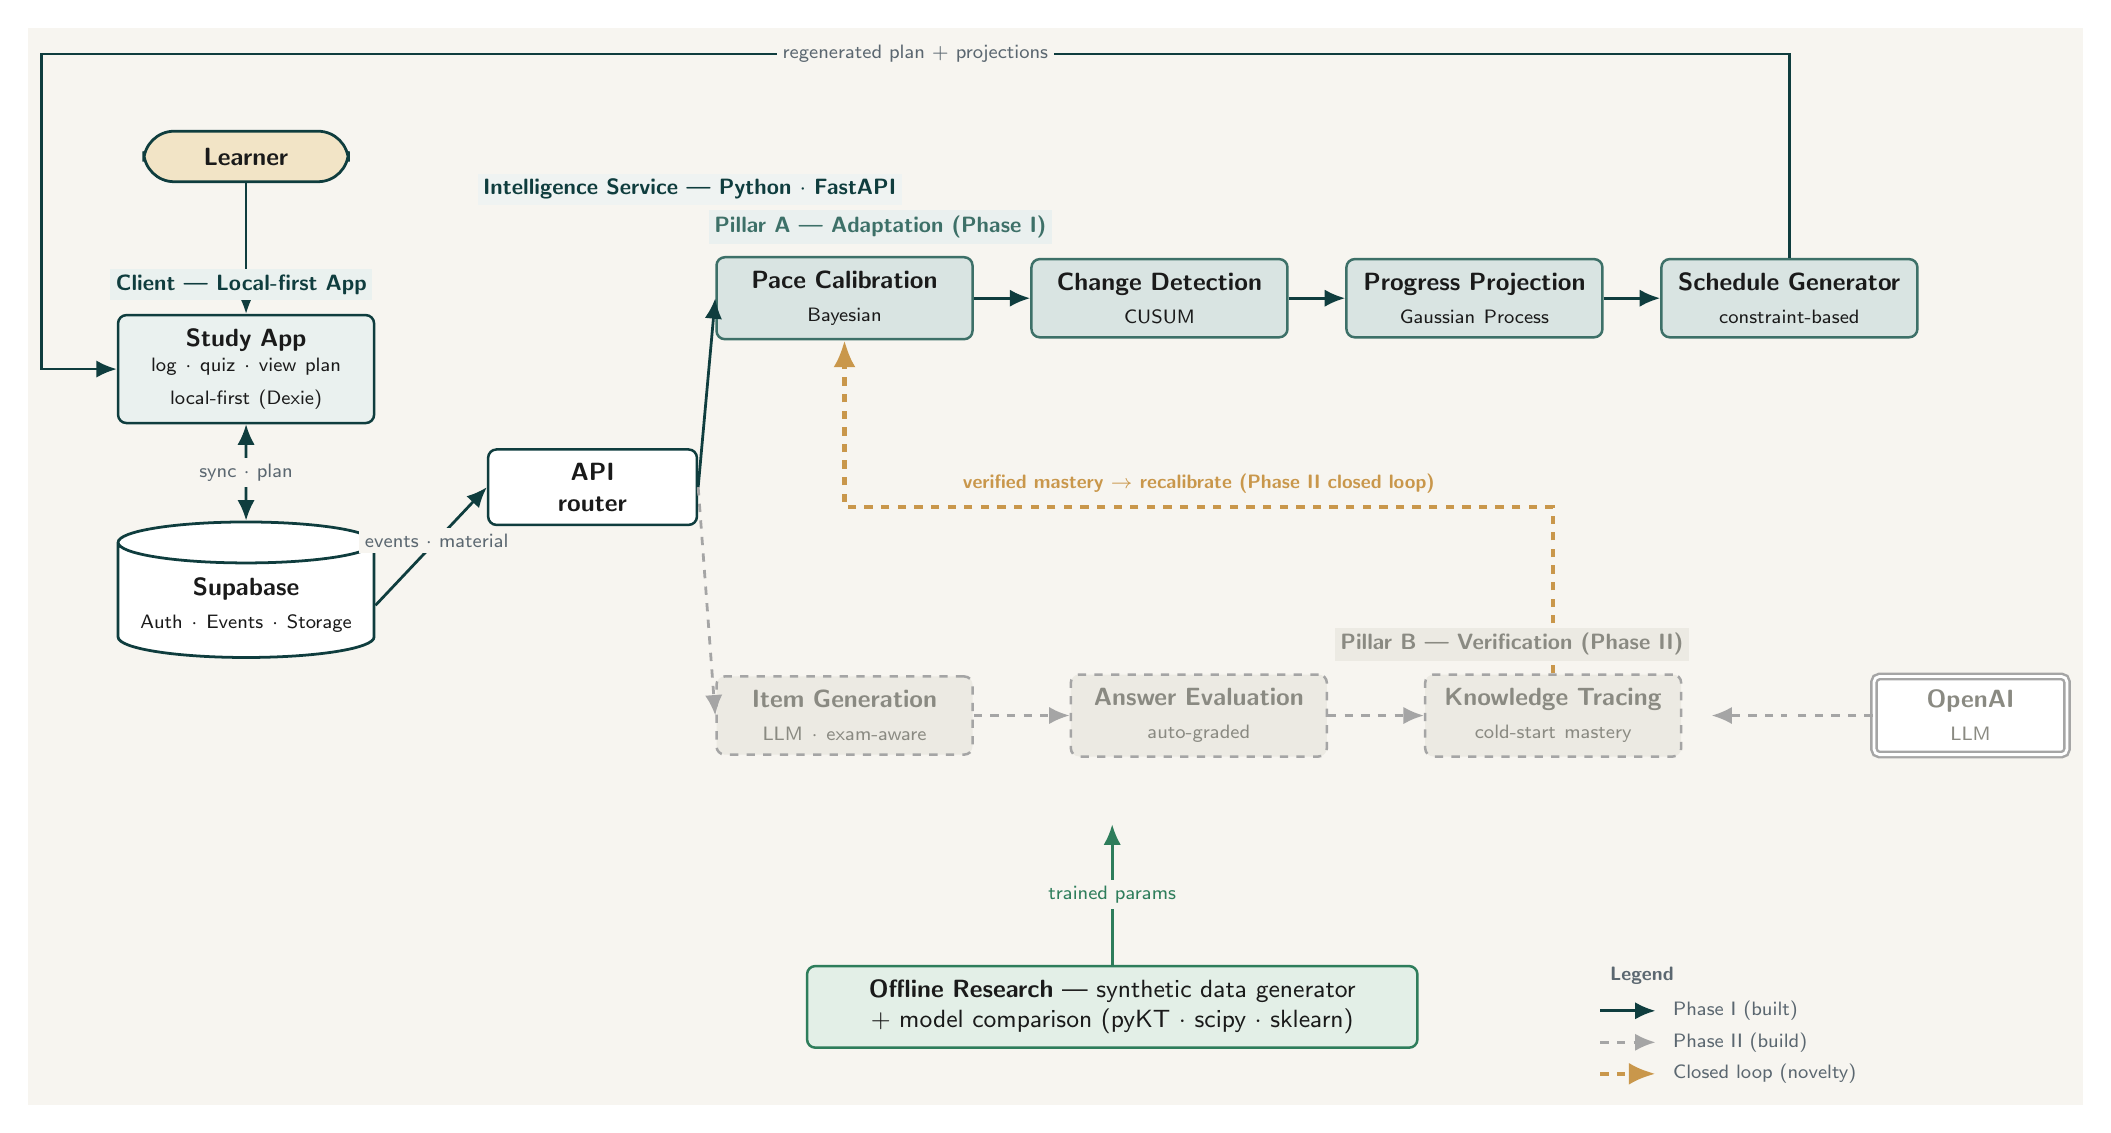
\begin{tikzpicture}[
  font=\small,
  every node/.style={text=ink},
  box/.style={rounded corners=3pt, draw, line width=0.9pt, align=center,
              inner sep=5pt, text width=2.9cm, fill=white},
  proc/.style={box, draw=tealMed, fill=paFill},
  phase2/.style={box, draw=grey, dashed, fill=greyFill, text=greyText},
  hub/.style={cylinder, shape border rotate=90, aspect=0.16, draw=tealStroke,
              line width=1pt, fill=white, align=center, inner sep=5pt,
              text width=2.9cm, minimum height=1.4cm},
  actor/.style={rounded corners=11pt, draw=tealStroke, line width=1pt,
                fill=goldFill, align=center, inner sep=6pt, minimum width=2.6cm},
  ext/.style={draw=grey, line width=0.9pt, double, double distance=1pt,
              rounded corners=2pt, align=center, inner sep=5pt,
              text width=2.1cm, fill=white, text=greyText},
  router/.style={box, draw=tealStroke, fill=white, text width=2.3cm},
  research/.style={box, draw=green, fill=greenFill, text width=7.4cm},
  title/.style={font=\footnotesize\bfseries},
  flow/.style={-{Latex[length=2.6mm,width=2.2mm]}, line width=1.0pt, draw=tealStroke},
  flowbi/.style={{Latex[length=2.6mm,width=2.2mm]}-{Latex[length=2.6mm,width=2.2mm]},
                 line width=1.0pt, draw=tealStroke},
  dflow/.style={-{Latex[length=2.6mm,width=2.2mm]}, line width=1.0pt, dashed, draw=grey},
  loop/.style={-{Latex[length=3.4mm,width=2.8mm]}, line width=1.5pt, dashed, draw=gold},
  lbl/.style={font=\scriptsize, fill=cream, inner sep=2pt, text=slate},
  dlbl/.style={font=\scriptsize, fill=cream, inner sep=2pt, text=greyText},
  show background rectangle,
  background rectangle/.style={fill=cream},
]

% ============================ NODES ======================================
\node[actor] (LEARNER) at (0,10.4) {\textbf{Learner}};
\node[box, draw=tealStroke, fill=clientFill] (APP) at (0,7.7)
  {\textbf{Study App}\\[1pt]\scriptsize log $\cdot$ quiz $\cdot$ view plan\\[1pt]\scriptsize local-first (Dexie)};
\node[hub] (SB) at (0,4.7) {\textbf{Supabase}\\[1pt]\scriptsize Auth $\cdot$ Events $\cdot$ Storage};
\node[router] (ROUTER) at (4.4,6.2) {\textbf{API}\\\textbf{router}};

% Pillar A lane (Phase I, solid) -- top, flows left -> right
\node[proc] (CAL)  at (7.6,8.6) {\textbf{Pace Calibration}\\[1pt]\scriptsize Bayesian};
\node[proc] (DET)  at (11.6,8.6) {\textbf{Change Detection}\\[1pt]\scriptsize CUSUM};
\node[proc] (PROJ) at (15.6,8.6) {\textbf{Progress Projection}\\[1pt]\scriptsize Gaussian Process};
\node[proc] (SCH)  at (19.6,8.6) {\textbf{Schedule Generator}\\[1pt]\scriptsize constraint-based};

% Pillar B lane (Phase II, greyed) -- bottom, flows left -> right
\node[phase2] (GEN)  at (7.6,3.3) {\textbf{Item Generation}\\[1pt]\scriptsize LLM $\cdot$ exam-aware};
\node[phase2] (EVAL) at (12.1,3.3) {\textbf{Answer Evaluation}\\[1pt]\scriptsize auto-graded};
\node[phase2] (KT)   at (16.6,3.3) {\textbf{Knowledge Tracing}\\[1pt]\scriptsize cold-start mastery};

% External + research
\node[ext] (OAI) at (21.9,3.3) {\textbf{OpenAI}\\[1pt]\scriptsize LLM};
\node[research] (RES) at (11.0,-0.4)
  {\textbf{Offline Research} --- synthetic data generator $+$ model comparison (pyKT $\cdot$ scipy $\cdot$ sklearn)};

% ====================== CONTAINER BOXES (background) =====================
\begin{scope}[on background layer]
  \node[draw=tealStroke, line width=1pt, rounded corners=6pt, fill=clientFill,
        fit=(APP), inner sep=10pt] (clientBox) {};
  \node[draw=tealMed, line width=1pt, rounded corners=6pt, fill=paFill!55,
        fit=(CAL)(DET)(PROJ)(SCH), inner sep=10pt] (paBox) {};
  \node[draw=grey, dashed, line width=1pt, rounded corners=6pt, fill=greyFill,
        fit=(GEN)(EVAL)(KT), inner sep=10pt] (pbBox) {};
  \node[draw=tealStroke, line width=1.1pt, rounded corners=7pt, fill=svcFill,
        fit=(ROUTER)(paBox)(pbBox), inner sep=13pt] (svcBox) {};
\end{scope}

% ============================ EDGES ======================================
\draw[flow] (LEARNER) -- (APP);
\draw[flowbi] (APP) -- (SB) node[lbl, midway]{sync $\cdot$ plan};
\draw[flow] (SB.east) -- (ROUTER.west) node[lbl, pos=0.55]{events $\cdot$ material};

% router into the two lanes
\draw[flow]  (ROUTER.east) -- (CAL.west);
\draw[dflow] (ROUTER.east) -- (GEN.west);

% Pillar A pipeline
\draw[flow] (CAL)  -- (DET);
\draw[flow] (DET)  -- (PROJ);
\draw[flow] (PROJ) -- (SCH);

% Pillar B pipeline
\draw[dflow] (GEN)  -- (EVAL);
\draw[dflow] (EVAL) -- (KT);

% OpenAI feeds Pillar B
\draw[dflow] (OAI) -- (pbBox.east) node[dlbl, pos=0.5]{};

% Schedule -> App (plan return, up over the top via far-left lane)
\draw[flow] (SCH.north) -- (19.6,11.7) -- (-2.6,11.7) -- (-2.6,7.7) -- (APP.west);
\node[lbl] at (8.5,11.7) {regenerated plan $+$ projections};

% Research -> service (trained params)
\draw[flow, draw=green] (RES.north) -- (RES.north|-svcBox.south);
\node[lbl, text=green] at ($(RES.north)!0.5!(RES.north|-svcBox.south)$) {trained params};

% closed loop: verified mastery -> calibration (right->left through centre gap)
\draw[loop] (KT.north) -- (16.6,5.95) -- (7.6,5.95) -- (CAL.south);
\node[font=\scriptsize\bfseries, fill=cream, inner sep=2pt, text=gold]
      at (12.1,6.25) {verified mastery $\rightarrow$ recalibrate  (Phase II closed loop)};

% ---- container titles (on top so arrows pass behind) ---------------------
\node[title, text=tealStroke, fill=clientFill, inner sep=2pt, anchor=west]
      at ([xshift=8pt]clientBox.north west) {Client --- Local-first App};
\node[title, text=tealStroke, fill=svcFill, inner sep=2pt, anchor=west]
      at ([xshift=10pt]svcBox.north west) {Intelligence Service --- Python $\cdot$ FastAPI};
\node[title, text=tealMed, fill=paFill!55, inner sep=2pt, anchor=west]
      at ([xshift=8pt]paBox.north west) {Pillar A --- Adaptation (Phase I)};
\node[title, text=greyText, fill=greyFill, inner sep=2pt, anchor=east]
      at ([xshift=-8pt]pbBox.north east) {Pillar B --- Verification (Phase II)};

% ---- legend (bottom-right) -----------------------------------------------
\begin{scope}[shift={(17.2,-0.9)}]
  \node[anchor=west, font=\scriptsize\bfseries, text=slate] at (0,0.9) {Legend};
  \draw[flow] (0,0.45) -- (0.7,0.45);
  \node[anchor=west, font=\scriptsize, text=slate] at (0.8,0.45) {Phase I (built)};
  \draw[dflow] (0,0.05) -- (0.7,0.05);
  \node[anchor=west, font=\scriptsize, text=slate] at (0.8,0.05) {Phase II (build)};
  \draw[loop] (0,-0.35) -- (0.7,-0.35);
  \node[anchor=west, font=\scriptsize, text=slate] at (0.8,-0.35) {Closed loop (novelty)};
\end{scope}

\end{tikzpicture}
\end{document}
